\documentclass{report}
\title{\textsc{A Digital Signal Processing Report on \\ \Huge Image Steganography using LSB Matching}}
\author{\\\\ {\bf \underline{Member Details}} \\\\{\bf MEMBER-1: Himanshu Sharma} \\ {\bf Roll Number: $1610110149$} \\ {\bf Dept. of Electrical Engineering (ECE)} \\\\{\bf MEMBER-2: Mridul Agarwal} \\ {\bf Roll Number: $1610110199$} \\ {\bf Dept. of Electrical Engineering (EEE)} \\\\ {\bf MEMBER-3: Vedansh Gupta} \\ {\bf Roll Number: $1610110429$} \\ {\bf Dept. of Electrical Engineering (ECE)}\\\\\\\\ {\bf Shiv Nadar University,} \\ {\bf Gautam Buddh Nagar,  Greater Noida, Uttar Pradesh 201314} \\\\\\ \textsc{ Under the guidance of Professor Vijay K. Chakka}}
\date{}

\usepackage[margin=0.8in]{geometry}
\usepackage{graphicx}
\usepackage{float}
\usepackage{amsmath}
\usepackage{algorithm}
\usepackage[noend]{algpseudocode}
\usepackage{fourier-orns}

\begin{document}
\maketitle
\pagenumbering{gobble}
\renewcommand{\thesection}{\arabic{section}}
% include the paper here.
\section{Paper Comprehension by Member 1 - Himanshu Sharma}
{\it Image Steganography} is the art of hiding information inside a digital image. Steagnography does not restrict to only plain text but it includes text, video, audio and image hiding also. In this report, the author has restricted himself to text data type only. Even when doing text embedding, there are immense possible algorithms to choose from. The most popular among them is the LSB replacement or Least Significant Bit replacement. With this type of algorithm, the least significant bit of each pixel (only one channel out of the RGB pallete) is changed by a bit decided according to the message bit. Therefore, we should not expect much change in the image after data hiding because the least significant bit is changed. For example, lets take a blue channel with value of 145. In binary, it is equivalent of 10010001. If by some technique, the last bit is changed to 0, then the decimal equivalent would become 144, which does not change the image much. This is the power of LSB replacement. It basically relies on the fact that hiding message bits in the LSB of each pixel does not affect the image much, in fact, the image practically remains as it is. There are, however, techniques now in modern signal processing science which can detect that some data is hidden in the image or not, a field called {\it steganalysis}. A successful hiding algorithm would be that, that would allow high payload and still look similar to the original image. 

\subsection{LSB Matching}
In LSB matching, if the message bit does not match with the pixel's LSB, then $\pm 1$ is randomly added to that pixel value. Unlike LSB replacement, where the pixel's LSB is just replaced by the message bit, here, a set of conditions are used to modify the pixel. LSB Matching could not be detected using the techniques used to detect LSB replacement. However, now it has been proved that LSB matching acts like a low pass filter on the digital images and therefore, this fact is utilized to detect whether LSB matching is applied on an image or not. \par Usually, two consecutive pixels are taken alongwith two consecutive message bits. The consecutive pairs are chosen randomly based on the {\it pseudo-random number generator} (PRNG). If the LSB matching is used as it is, then any pixel could be chosen with every pixel pair having equal chances of being selected by the algorithm. This has a flaw. This type of approach makes it difficult to disguise a changed pixel to the pixel surrounding it. For example, if lot of pixels are changed in a close vicinity, then they could be easily identified if the region is light in color, like sky which is light blue in color. The paper chosen here tries to rectify this problem by chosing those pixels on the image which lie on the edges. Edges are usually sharper than the surrounding regions and therefore its not easy to identify the change in pixel color on the edges. Similar papers have already been published. All of them suggest to use what is called the {\it pixel-value difference} (PVD). \par In PVD, what we do is that when we try to hide a message bit in a pixel's LSB, the pixel value is compared with its neighbouring pixels. If the difference is large, then more bits can be accomodated in that region without them being easily identified. Why? Because if there is a large difference in the pixel values then on changing the pixel value will not generate any significant difference. For example, if a pixel that is to be modified has a value of 45 and it's neighbouring pixel has a value of 145, then the difference $\displaystyle \Delta = 145-45=100$. Now, if by some technique if this pixel value if changed to 46, then the difference would become $\displaystyle \Delta' = 145-46 = 99$. To a human eye, this difference is not accountable. PVD is a good approach, in fact, far more better that PRNG because it utilizes the fact that sharp changes can be used to hide the information. \par In both LSB replacement and LSB matching, a travelling order is generated using PRNG which also acts as a key for decoding the stego-image. In both of these algorithms, the LSB of the selected pixel becomes equal to the message bit. According to the algorithm, if the two consecutive pixels are $x_{i}$ and $x_{i+1}$ and the consecutive message bits are $m_{i}$ and $m_{i+1}$, then the pixels are modified such that $x_{i}$ becomes $x_{i}^{'}$ and $x_{i+1}$ becomes $x_{i+1}^{'}$ and the following relation holds.
\begin{center}
$ \displaystyle LSB(x_{i}^{'})=m_{i} \textrm{ and } LSB \Big( \Big\lfloor{\frac{x_{i}^{'}}{2}}\Big \rfloor + x_{i+1}^{'} \Big) = m_{i+1}$
\end{center}
From experiments done by the authors of the paper it has been shown that even if the cover image has rough textures, it will still have smooth regions in every $5 \times 5$ non-overlapping blocks. So, if by any chance, a pixel is selected in that region for message hiding then it could be easily identified. This is what the paper aims to solve.

\subsection{Bit Planes}
We now come to a brief discussion on what is called the bit planes. Bit planes help us visualize the importance of the significant bits used to represent the images. They clearly display the fact that altering the LSB of pixels is less damaging to the original image than altering the MSB of the same original image. Before we discuss them in great detail, let me show an example. Suppose we have a cover image which is shown below.

\begin{figure}[H]
\centering

\includegraphics[width=0.5\textwidth]{images/desktop.jpg}
\caption{Cover Image}
\end{figure}
Its bit planes are shown below. The LSB plane and the MSB planes are what we display first.
\begin{figure}[H]
\centering
\begin{minipage}{0.46\linewidth}
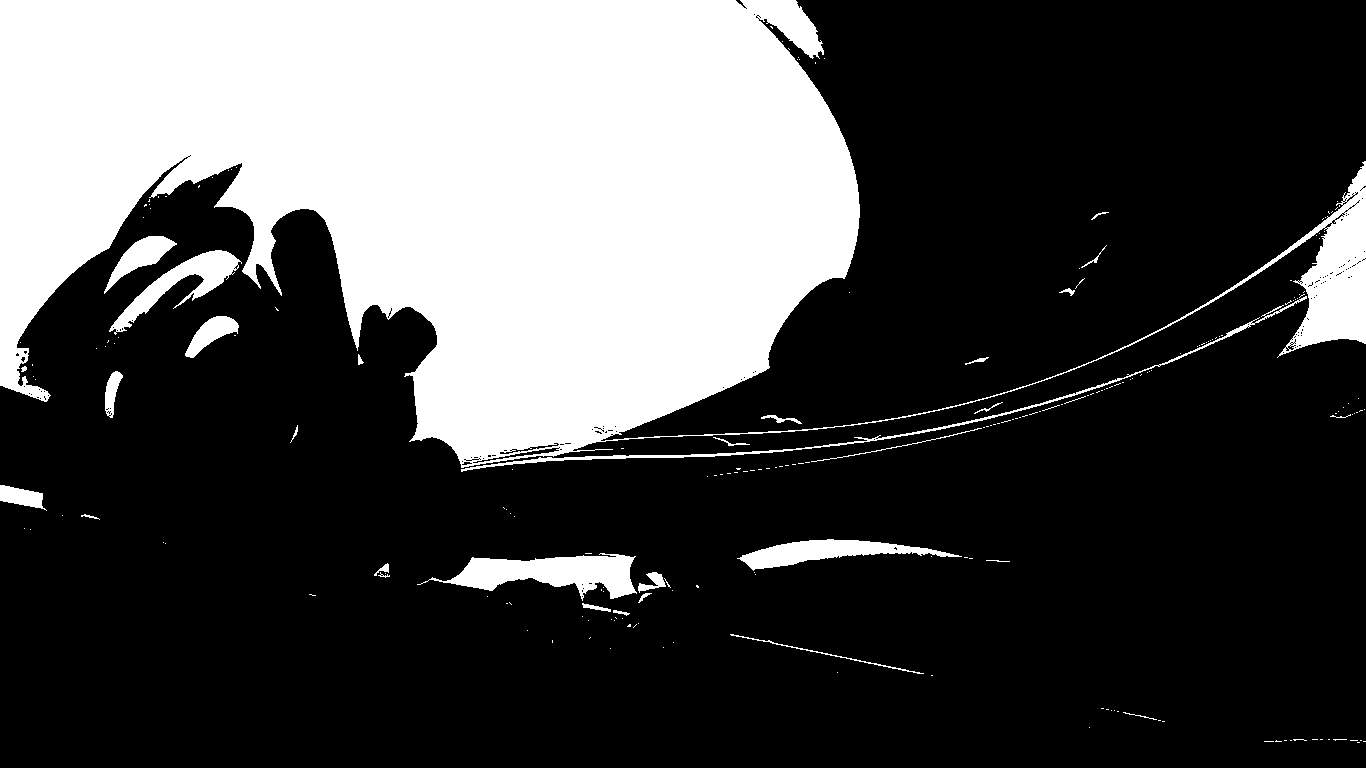
\includegraphics[width=\textwidth]{images/plane1.png}
\caption{MSB Plane}
\end{minipage}
\hfill
\begin{minipage}{0.46\linewidth}
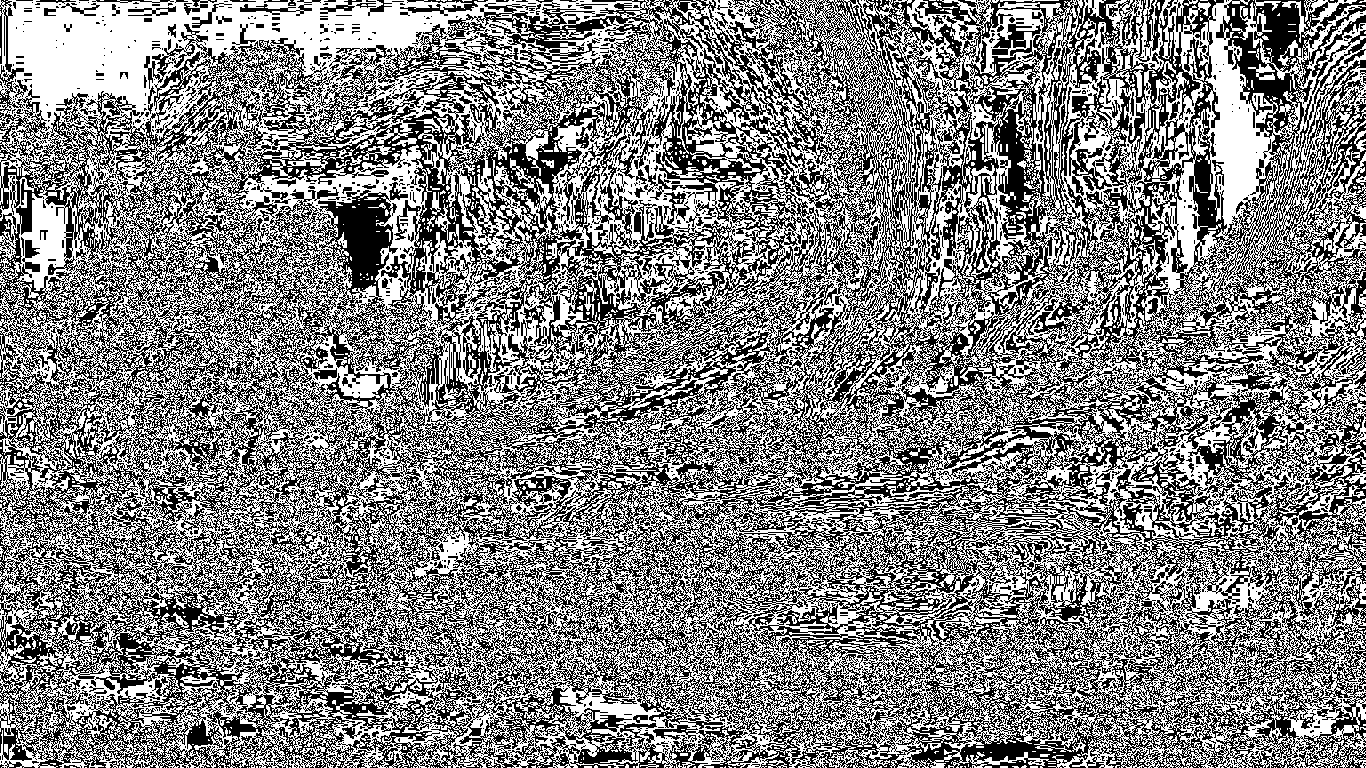
\includegraphics[width=\textwidth]{images/plane8.png}
\caption{LSB Plane}
\end{minipage}
\end{figure}

Changing a pixel value in the MSB plane is more prone to human eye detection as compared to the LSB plane. This is because a MSB plane has more structured black and white regions, and so, changing any pixel value, for example say, that a pixel is changed from white to black in the white region, then it would be easily detected. Whereas, on a LSB plane, the black and white regions are more uniformly aligned, just like {\it white noise} on a television screen. Inverting any color on the LSB plane won't change the visual effect. Hence, it is always advised to change the LSB plane in stegnography.
\par The idea is to generate these images using single values. Since we have 3 values associated with a single pixel {\it (R, G, B)}, it would be a great idea to convert the image to a grayscale image, so that each pixel is represented by a single value. Now each pixel value, which initially was a three dimensional array, is converted to a one dimensional array having a single value. This matrix of single values (grayscale image) is passed to a function which converts these decimal pixel values to 8 bit binary number. As per the request of the user, the $i^{th}$ bit from each binary pixel is accessed. So, for example, if a pixel has 8-bit binary representation as 11110101 and the user asks for fifth bit plane, then the fifth bit from starting would be accessed and that is 0 for this example. These values are stored in another matrix. So now we have a matrix with only 1 and 0s. We now multiply each and every value of the matrix by 255. The matrix becomes full of 255 and 0s. Zero represent black color and 255 represent white color. When saved, this image is a black and white $i^{th}$ bit plane. 

\par Below, I have shown all the bit planes of the above cover image.
\begin{figure}[H]
\centering
\begin{minipage}{0.46\linewidth}
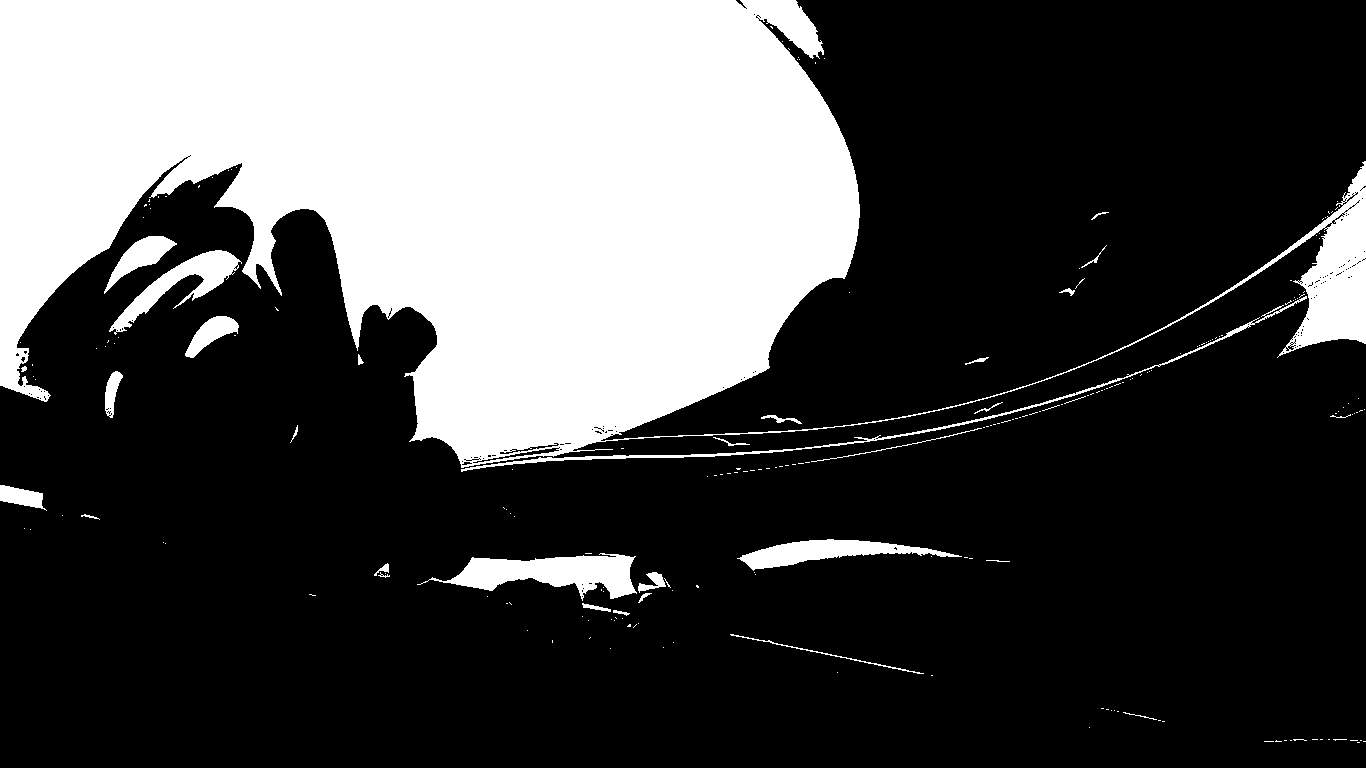
\includegraphics[width=\textwidth]{images/1.png}
\caption{$1^{st}$ bit plane or the MSB Plane}
\end{minipage}
\hfill
\begin{minipage}{0.46\linewidth}
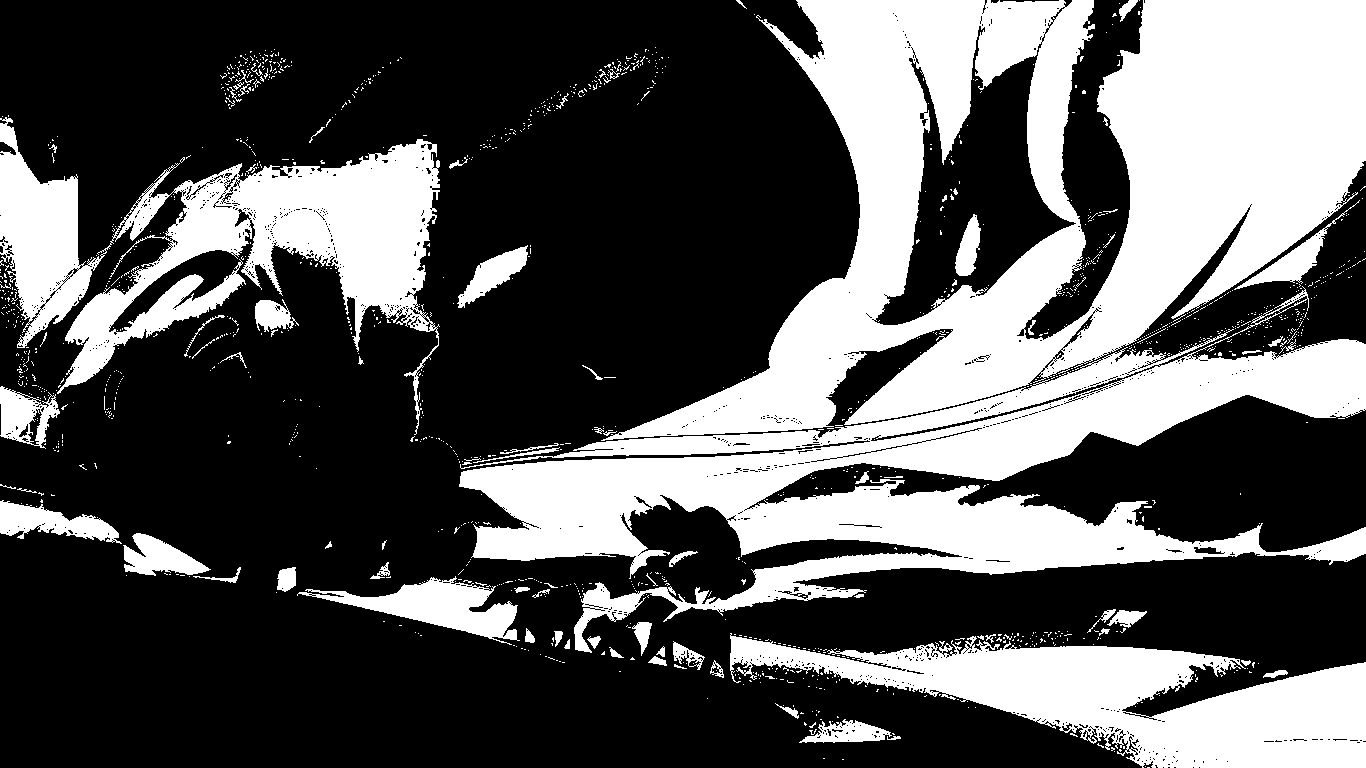
\includegraphics[width=\textwidth]{images/2.png}
\caption{$2^{nd}$ bit plane}
\end{minipage}
\vfill
\begin{minipage}{0.46\linewidth}
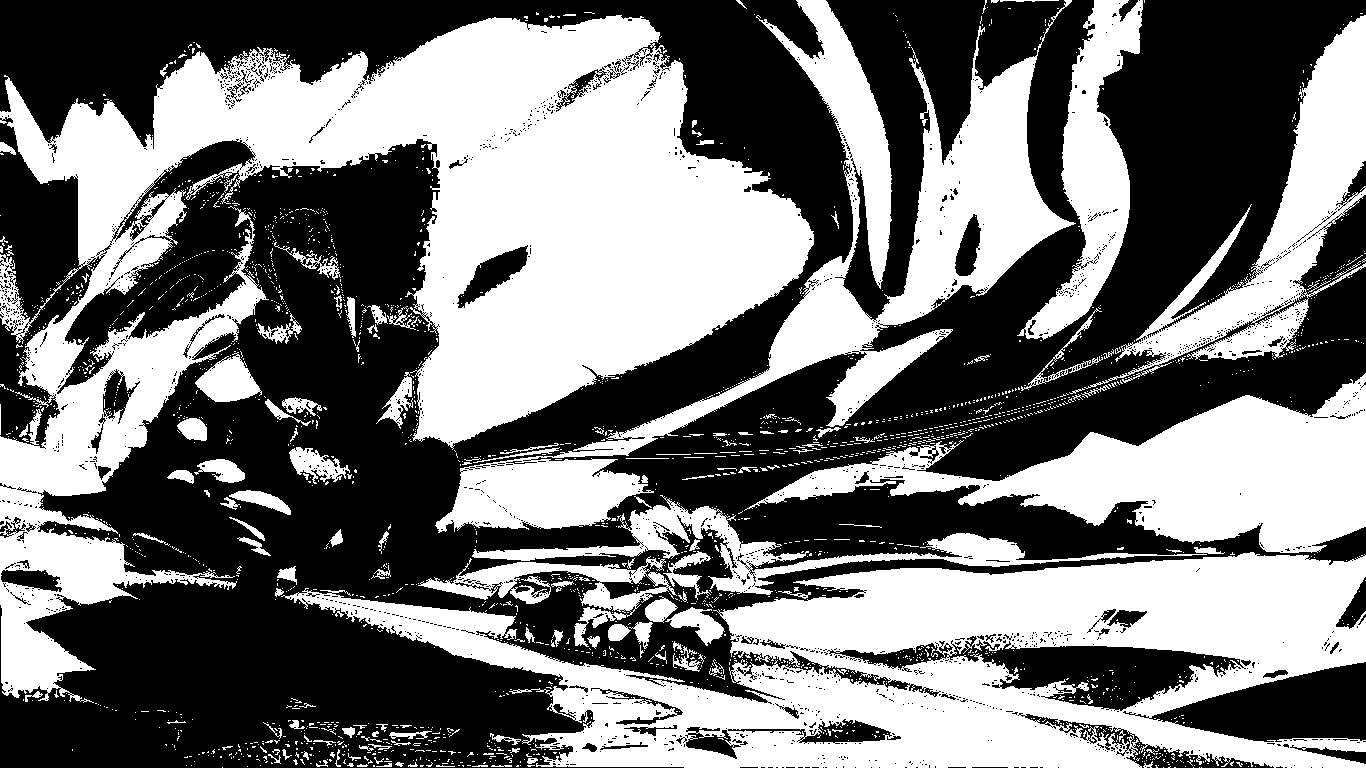
\includegraphics[width=\textwidth]{images/3.png}
\caption{$3^{rd}$ bit plane}
\end{minipage}
\hfill
\begin{minipage}{0.46\linewidth}
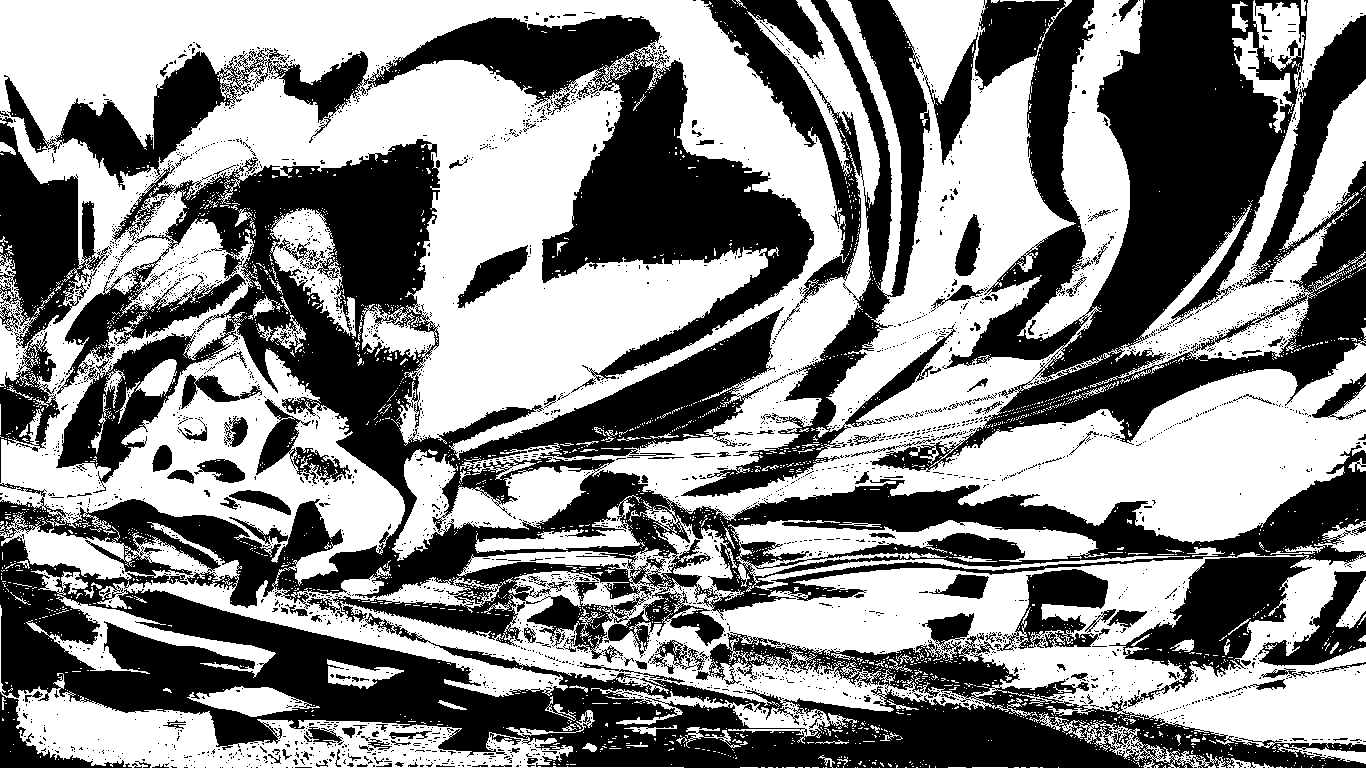
\includegraphics[width=\textwidth]{images/4.png}
\caption{$4^{th}$ bit plane}
\end{minipage}
\hfill
\begin{minipage}{0.46\linewidth}
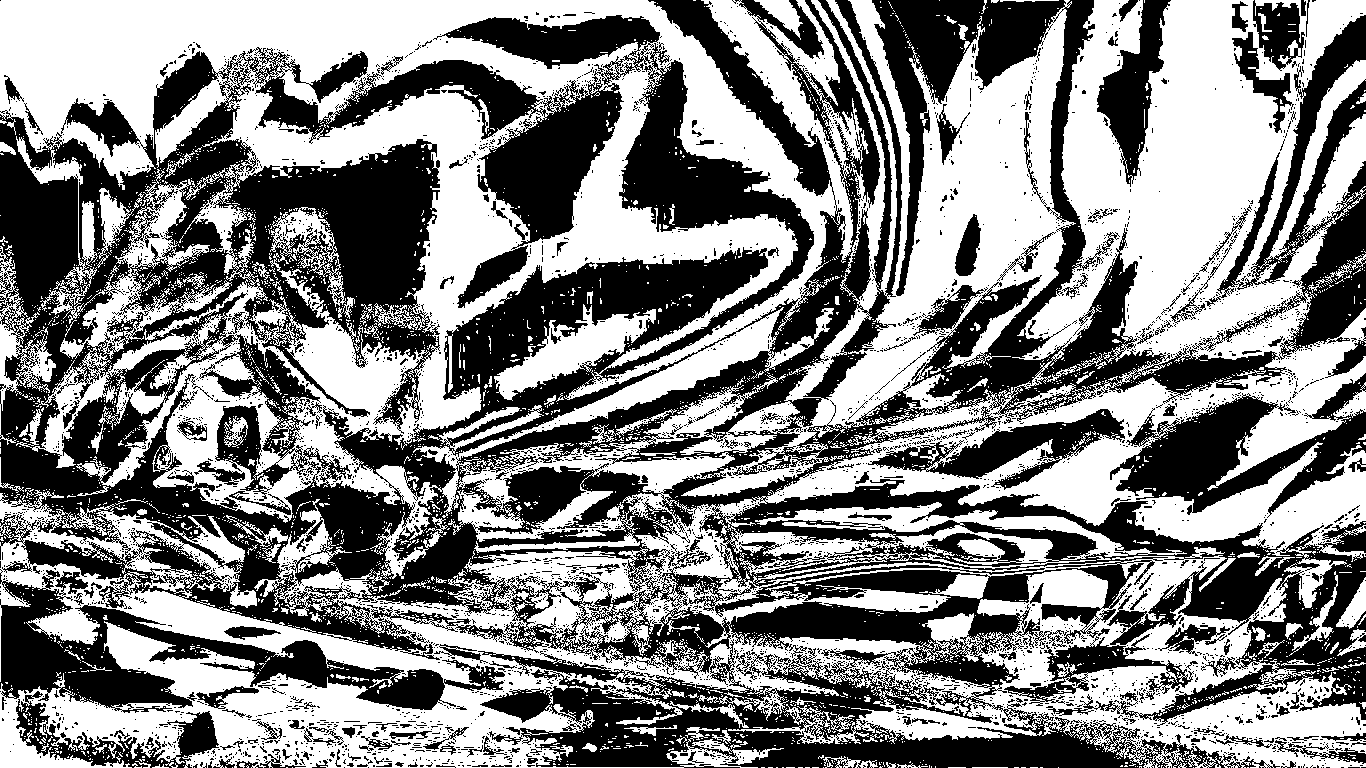
\includegraphics[width=\textwidth]{images/5.png}
\caption{$5^{th}$ bit plane}
\end{minipage}
\hfill
\begin{minipage}{0.46\linewidth}
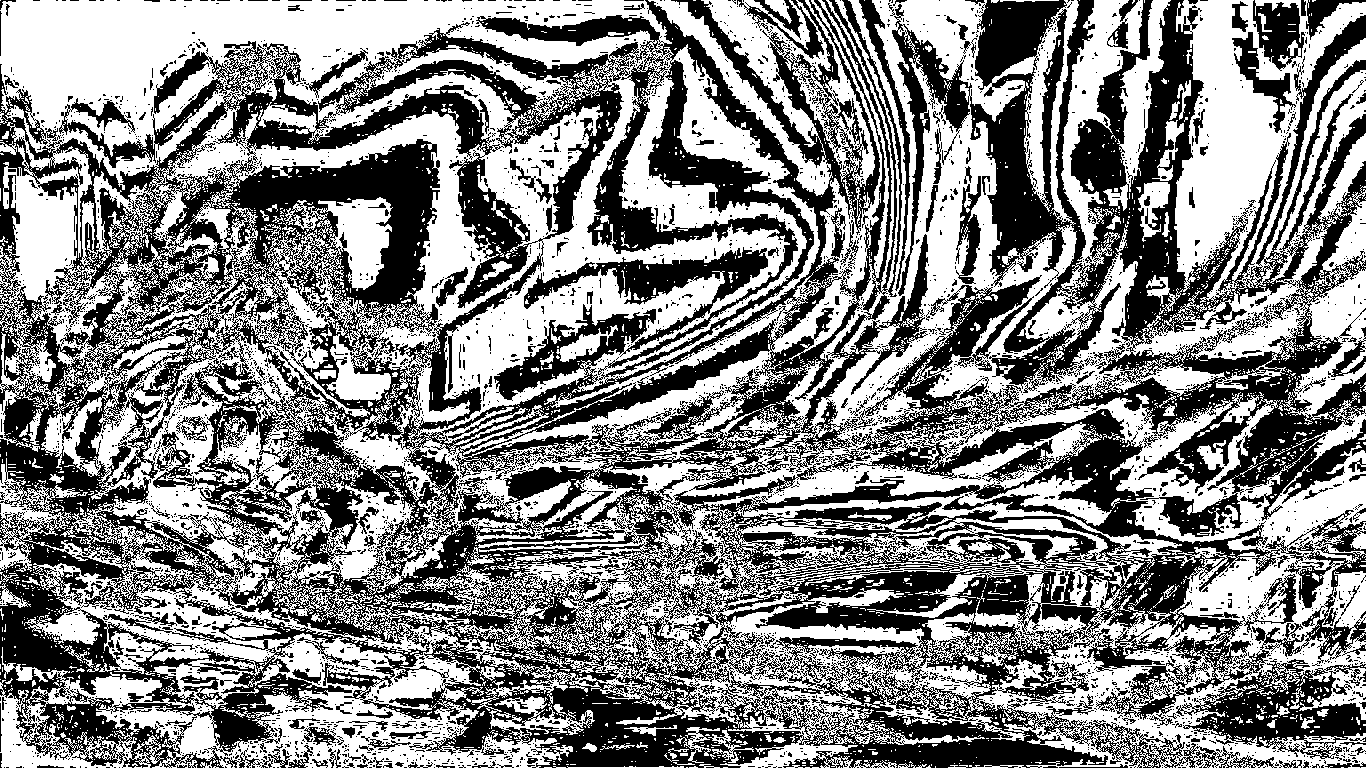
\includegraphics[width=\textwidth]{images/6.png}
\caption{$6^{th}$ bit plane}
\end{minipage}
\hfill
\begin{minipage}{0.46\linewidth}
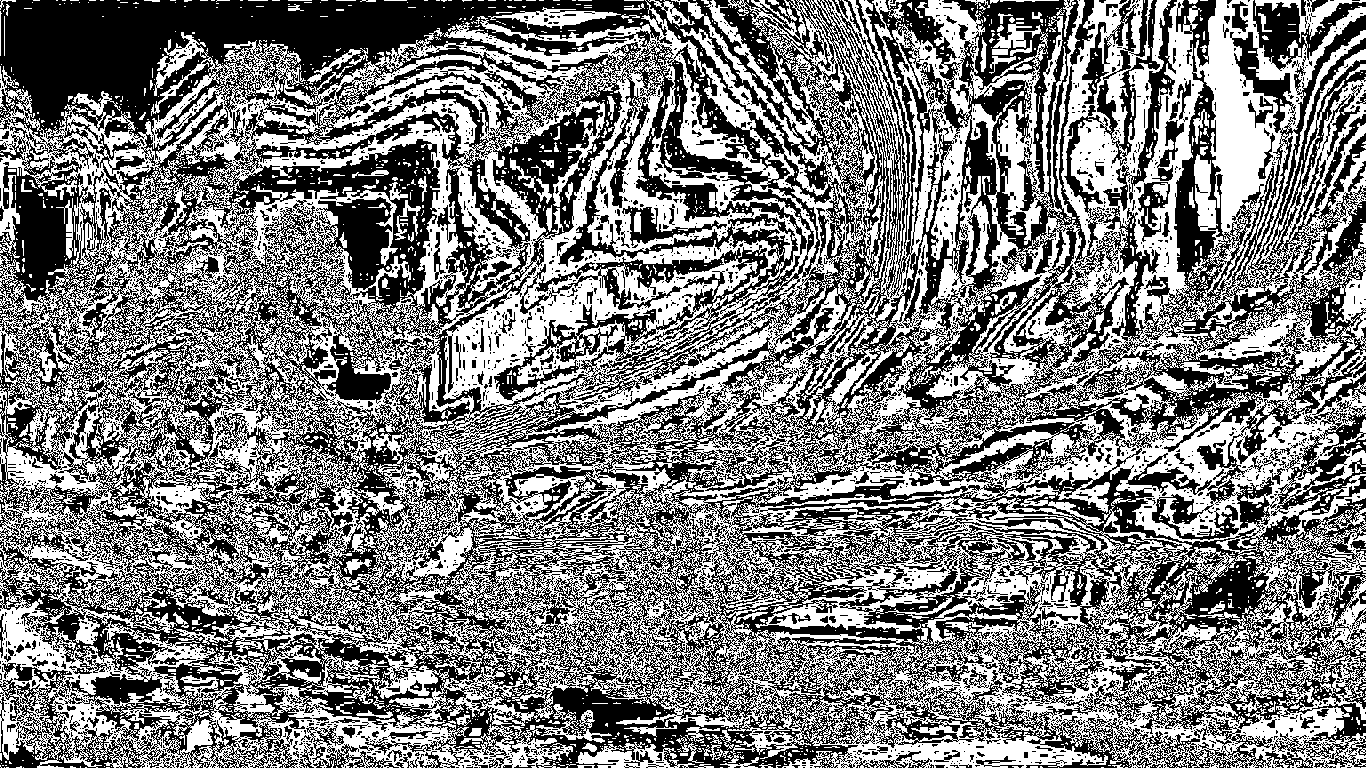
\includegraphics[width=\textwidth]{images/7.png}
\caption{$7^{th}$ bit plane}
\end{minipage}
\hfill
\begin{minipage}{0.46\linewidth}
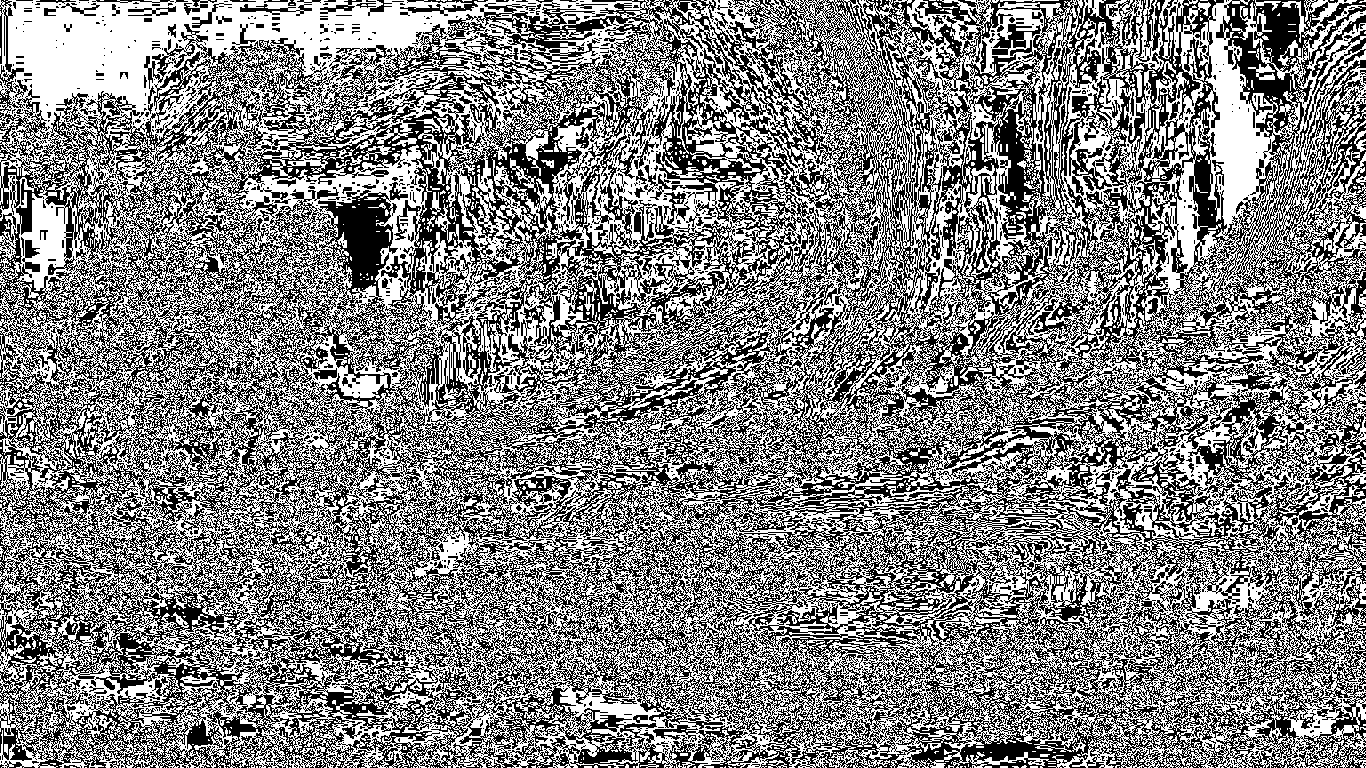
\includegraphics[width=\textwidth]{images/8.png}
\caption{$8^{th}$ bit plane or the LSB plane}
\end{minipage}

\end{figure}
Clearly, as we increase the bit plane number, we are bound to get more better results. Increasing the bit plane number implies less human eye detection in case of a pixel change. Now let us see the mathematical reasoning behind the bit planes. \newpage Let us define a closed form expression which converts a binary number to its decimal equivalent.
\begin{equation}
\displaystyle d(n) =\sum_{i=1}^{n}g(n+1-i,\textrm{ } b)2^{n-i}
\end{equation}
where $g(k, b)$ returns the $k^{th}$ bit from left of the binary number $b$ and $n$ denotes the length of the binary number. Here we are dealing with $n=8$. Let us say that the $j^{th}$ bit is changed while doing some steganography. The $j^{th}$ bit could be LSB or MSB or any other bit in between, we are not concerned about that for now. So, we know that $ 1 \leq j \leq n$. Let the original binary number be $\alpha$ and the binary number after the changed bit be denoted by $\beta$. Hence we get,

\begin{center}
$\displaystyle d_{1}(n) =\sum_{i=1}^{n}g(n+1-i,\textrm{ } \alpha)2^{n-i}$ and
$\displaystyle d_{2}(n) =\sum_{i=1}^{n}g(n+1-i,\textrm{ } \beta)2^{n-i}$
\end{center}
If we take the difference $\Delta d(n) = (d_{1} - d_{2})(n)$, the we get,
\begin{equation}
\displaystyle \Delta d(n) =\sum_{i=1}^{n}g(n+1-i,\textrm{ } \alpha)2^{n-i} - \sum_{i=1}^{n}g(n+1-i,\textrm{ } \beta)2^{n-i}
\end{equation}
Assuming all other bits of $\alpha$ and $\beta$ to be same except for the $j^{th}$ bit, we get,
\begin{center}
$\displaystyle \Delta d(n) = g(n+1-j, \alpha)2^{n-j} - g(n+1-j, \beta)2^{n-j} = 2^{n-j} \Delta g(n, j)$ 
\end{center}
where, $\Delta g(n, j) = g(n+1-j, \alpha) - g(n+1-j, \beta)$ and thus we get,
\begin{equation}
\displaystyle \delta (n) = |\Delta d(n)| = 2^{n-j}|g(n, j)|
\end{equation}

Note that $\Delta d(n)$ is the difference in the decimal values of the binary numbers which can be positive, negative or 0, $\delta (n)$ is always non-negative. Now, $|\Delta g(n, j)|$ can be defined as follows;
\[
|\Delta g(n, j)| = 
\begin{cases}
1, & j^{th} \text{ bit of $\alpha$ and $\beta$ are different} \\
0, & \text{otherwise}
\end{cases}
\]
The {\it otherwise} case is trivial because if there is no difference in even the $j^{th}$ bit of these binary numbers, then both of them are identical. This means that the number was not changed. But if the number has change, then $|\Delta g(n, j)|$, for sure, is 1. Now, it is in this part we are concerned with the difference. We need to minimize this difference $\delta(n)$ because then only our stego-image will be statistically close to the original image. The value of $\delta(n)$ could be minimum only if $n=j$ (see equation 3), i.e., $\delta(n) = |\Delta g(n, j)|$ which is 1 if we assume that the pixel bit was changed. That is, the difference in decimal value has the minimum magnitude of 1, 0 being the trivial case that the binary numbers were never changed. Since the decimal difference value will decide the grayscale of the stego-image, we want to minimize it. This proves that if we want statistically similar features in the stego-image, we should take $j=n$, i.e., we should consider the LSB only, because that would affect the orignal decimal value by $\pm 1$ only. \par If we do consider $j=1$, then $\delta(n) = 2^{n-1} |\Delta g(n, 1)|$. Again, $\Delta g(n, 1) = \pm 1$ if we consider that the pixel value was changed. However, it is clear that $2^{n-1}$ will yield the maximum difference, and therefore, $j=1$ should never be taken, or, MSB should never be changed.

\subsection{The Algorithm}
The paper provides a scheme to optimize the traditional LSB algorithm. It covers an extra mile by embedding the key information in the stego-image itself. We can also say that first the pixels are changed according to the algorithm and then the key information is embedded into the image. Finally, the image thus obtained is the stego-image. \par Let me now explain how the data embedding is done in the image.
\newpage
\underline{\large Data Embedding} \\
\par Data embedding in the image starts by a new process which is generally not found in traditional steganography algorithms. First the image is divided into non-overlapping blocks of size $B \times B$ (as per the paper). Then we rotate each and every individual block by some random angle $\theta$, where $\theta \in \{0, 90, 180, 270\}$ in degrees. \par Dividing the image into non-overlapping blocks and then rotating each block by a random angle increases the security. That is because if we rotate the image before we embedd message bits in it and then later on rotate back those blocks to form the cover-like image, we have actually gained a great deal of security as compared to the image on which the embedding was done directly. Think about it, since the image is rotated back after embedding, all the embedded bits have been shuffled. Now, if some attacker tries to bruteforce, then even if he guesses the correct key, he won't be able to get the correct message. \par Now, the image is raster scanned. Raster scan is like converting an image into a row vector. In language like Python which I am using, this transformation can be achieved by using the statement \texttt{img.flatten()}, where \texttt{img} is the image as a numpy array. To read about numpy, please visit the docs. After this step, consecutive pixels are selected in pairs and following set is defined.
\begin{equation}
S(t) = \{(x_{i}, x_{i+1})| |x_{i} - x_{i+1}| \geq t, \forall (x_{i}, x_{i+1}) \in V \}
\end{equation}
where $V$ is the raster scanned image and $t$ is some value in the set $\{0, 1, 2, ..., 31 \}$. In other words, $S(t)$ is the set of all those consecutive pixels in the raster scanned image which have a differece greater than or equal to the parameter $t$. After this, the threshold value $T$ is calculated by the following method.
\begin{equation}
T = \textrm{argmax}_{t}\{2 \times n(S(t)) \geq n(M)\}
\end{equation}
where, $n(S)$ denotes the number of elements in $S$ and $M$ is the message. This equation, that is, equation 5 checks whether the message bits can be embedded in the image or not. Now let us understand what this equation actually means. Suppose a hypothetical case of $S(t) = \{ (x_{1}, x_{2}), (x_{3}, x_{4}), (x_{5}, x_{6}) \}$ for some $t=t_{1}$ and let $M$ be a 5 bit stream. Then, we find that $2 \times 3 \geq 5$ where $n(S(t)) = 3$. We chose some other $t$ now which is $t=t_{2} > t_{1}$. For this, let us say that we get $n(S(t)) = 2$, impling $2 \times 2 \geq 5$ which is false and therefore $T=t_{1}$. This is what equation 5 tries to say. It gives us that maximum $t$ for which the condition in the equaiton holds true. It is clear why we are multiplying by $2$. Thats because each pixel can hold one bit from the message stream and $S$ contains a tuple of such pixels. In total, we have twice the length pixels.	A good observation is that if $T=0 \textrm{ }\exists \textrm{ }t$, then that would mean that our equation 5 is satisfied only for max $t=0$. Hence, our equation 4 would become,
\begin{center}
$ S(0) = \{(x_{i}, x_{i+1})| |x_{i} - x_{i+1}| \geq 0, \forall (x_{i}, x_{i+1}) \in V \} $
\end{center}
This is what a conventional LSB steganography technique does. It just embedds the message stream without thinking about the difference between the consecutive pixels. \par We now come to the discusssion of the main pseudocode which actually embedds the data in the image. Below, I have shown the algorithm used for LSB matching.
\begin{algorithm}
\caption{LSB Matching}\label{euclid}
\begin{algorithmic}[1]
\Procedure{hide}{}
\If {$LSB(x_{i}) = m_{i}$} 
	\If {$f(x_{i}, x_{i+1})=m_{i+1}$}
	\State $(x_{i}^{'}, x_{i+1}^{'}) = (x_{i}, x_{i+1})$ 
	\Else 
	\State $(x_{i}^{'}, x_{i+1}^{'}) = (x_{i}, x_{i+1}+r)$ 
	\EndIf
\EndIf

\If {$LSB(x_{i})\neq m_{i}$}
	\If {$f(x_{i}-1, x_{i+1})=m_{i+1}$}
	\State $(x_{i}^{'}, x_{i+1}^{'}) = (x_{i}-1, x_{i+1})$
	\Else
	\State $(x_{i}^{'}, x_{i+1}^{'}) = (x_{i}+1, x_{i+1})$
	\EndIf
\EndIf
\EndProcedure
\end{algorithmic}
\end{algorithm}
\\ This algorithm is used for hiding the text data inside the image. $r$ is any random value in $\{ 1, -1\}$. Where, $(x_{i}^{'}, x_{i+1}^{'})$ are the new pixel values after data hiding. After this, the image blocks are rotated back to get the orignal image like image back and the angle values, the threshold $T$ and the block size are bundled into a binary file and returned as the key, back to the user. \newpage

\underline{\large Data Extraction} \\
\par Now, to get back the message stream, the image is first divided into blocks of size $B \times B$ again and then each of these blocks is rotated by the angles provided in the key file. Then those pixels are found in which data hiding was actually done using the inequality $|x_{i+1}-x_{i}|\geq T$. Now, to get back two units of the stream, the formula given in section 1.1 is used (refer section 1.1).

\subsection{Conclusions}
In the case of data embedding, the lower the value of $T$, more number of bits from the message can be embedded in the cover image. The following reasoning proves this; if we have two thresholds $T_{1}$ and $T_{2}$ with $T_{1} < T_{2}$, then this would mean 
\begin{center}
$\textrm{argmax}_{t}\{2 \times n(S_{1}(t)) \geq n(M)\} < \textrm{argmax}_{t}\{2 \times n(S_{2}(t)) \geq n(M)\}$
\end{center}
where,
\begin{center}
$ S_{1}(t) = \{ (x_{i}, x_{i+1})||x_{i} - x_{i+1}| > t_{1}, \forall (x_{i}, x_{i+1}) \in V\} $ \\
$ S_{2}(t) = \{ (x_{i}, x_{i+1})||x_{i} - x_{i+1}| > t_{2}, \forall (x_{i}, x_{i+1}) \in V\} $
\end{center} 
Because $T_{1} < T_{2} \implies t_{1} < t_{2}$ and that would mean that $S_{1}$ has lesser threshold value when compared to $S_{2}$. This would mean that more pixels would be available which satisfies $|x_{i} - x_{i+1}| > t_{1}$ than the pixels which satisfy $|x_{i} - x_{i+1}| > t_{2}$. Hence, $S_{1}$ would contain more elements or tuples than $S_{2}$. This is what the very first statement is saying, that if, threshold is small, more pixels could be accomodated. \par With steganography in mind, in general, we always need to compare the images for steganalysis. For this we first calculate the {\it mean square error} (MSE) between the cover $(A)$ and the stego-image $(B)$ by the following relation,
\begin{equation}
MSE(A, B) = \frac{1}{N} \sum_{i=0}^{N} (A_{i} - B_{i})^{2}
\end{equation}
Where, the subscript $i$ denotes the $i^{th}$ pixel of the image.
Here, actually, the MSE is the noise introduced in the cover image after steganography has been performed on it. So, in decibels (dB), the Peak Signal to Noise Ratio (PSNR) is given by,
\begin{equation}
PSNR_{dB} = 10 \log_{10}\Bigg|\frac{max^{2}(A)}{MSE}\Bigg|
\end{equation}
Where $max(A)$ is the maximum pixel value in the image or the peak signal available in the image. \par The techinque used in this paper produces exactly identical image after doing steganography as was the original cover image. Below, I have shown the eighth bit plane of a cover image and its stego-image as an example.
\begin{figure}[H]
\centering
\begin{minipage}{0.46\linewidth}
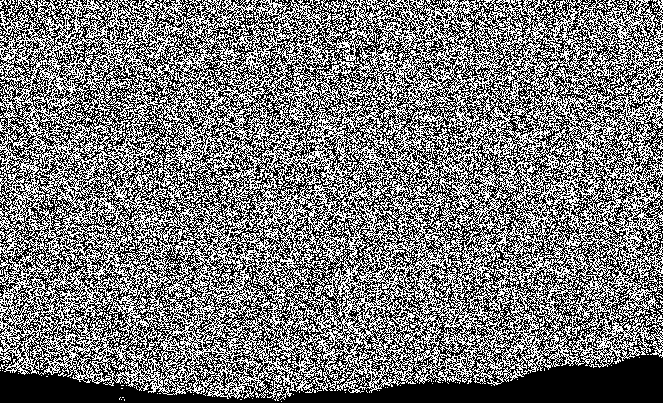
\includegraphics[width=\textwidth]{images/konsole.png}
\caption{Cover Image LSB plane}
\end{minipage}
\hfill
\begin{minipage}{0.46\linewidth}
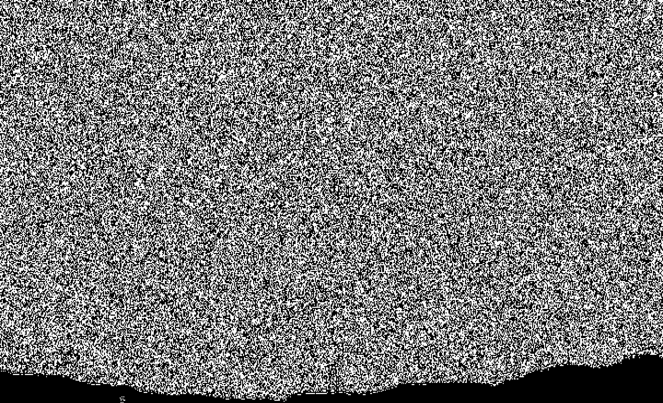
\includegraphics[width=\textwidth]{images/konsole-stego.png}
\caption{Stego Image LSB plane}
\end{minipage}
\end{figure}
Clearly, we see that both the bit planes are identical looking, although they are not in exact sense. If the planes are zoomed and then viewed, then it is easy to spot differences. These differences occur because of resizing done by the code and some due to the embedded text also. Since there is such an uniformity in the LSB planes of both cover and stego-image, its practically impossible for someone to spot the difference in the cover and stego-image. I thus conclude by saying that image steganography is successfully implemented by me. \underline{Full code base is written in Python and is  available on my GitHub repository at} \begin{center} {\bf https://github.com/hmnhGeek/DSP-Project-Report-LaTeX} \end{center}
This report is also available with it's complete \LaTeX code in the same repository under the \texttt{Report} folder. I would like the reader to surely go through the repository once.
\\
\par {\bf My contributions include the following,}
\begin{enumerate}
\item Full code base in Python dedicated to this project.
\item Report writing done with \LaTeX. 
\end{enumerate}

\section{Paper Comprehension by Member 2 - Mridul Agarwal}
The science which deals with the hidden communication is called steganography  whereras steganlaysis aims to detect the presence of hidden secret message in the stego media. There are different kinds of steganographic techniques which are complex and which have strong and weak points in hiding the information in various file formats. The file format used in this paper is images. The images which are used to hide the message $(M)$ are called cover images whereas the altered (steganographed) images are called stegos. The message hidden here is a binary stream. \par A steganography method is secure only when the statistics of the cover image and the stego are similar to each other. Image steganography is of two types-lossy compression and lossless compression. Lossy compression may not preserve the original image where as lossless compression preserves the original image. Examples of lossless compression formats are GIF,BMP,PNG etc. and that of lossy compression are JPEG. Also embedding capacity is also an important factor in designing a steganographic algorithm. \par Most of the existing steganographic techniques, the choice of embedding positions within a cover image mainly depends on a pseudorandom number generator (PRNG) without considering the relationship between the image content itself and the size of the secret message. Here the researchers have extended the LSB matching revisited (LSBMR) image steganography and propose an edge adaptive scheme which can select the embedding regions according to the size of secret message and the difference between two consecutive pixels in the cover image.
\subsection{LSB Replacement}
In this embedding technique, only the LSB of the cover image pixel is overwritten with the secret bit stream according to a pseudorandom number generator (PRNG). As a result, some structural asymmetry is introduced, and thus it is very easy to detect the existence of hidden message even at a low embedding rate.
\subsection{LSB Matching (LSBM)}
LSB matching (LSBM) employs a minor modification to LSB replacement. If the secret bit does not match the LSB of the cover image, then $\pm 1$ is randomly added to the corresponding pixel value. Statistically, the probability of increasing or decreasing for each modified pixel value is the same and so the obvious asymmetry introduced by LSB replacement can be easily avoided. Therefore, the common approaches used to detect LSB replacement are totally ineffective at detecting the LSBM.
\subsection{LSB Matching Revisited}
Unlike LSB replacement and LSBM, which deal with the pixel values independently, LSB matching revisited (LSBMR) uses a pair of pixels as an embedding unit, in which the LSB of the first pixel carries one bit of secret message, and the relationship (odd–even combination) of the two pixel values carries another bit of secret message. \par The regions located at the sharper edges present more complicated statistical features and are highly dependent on the image contents. It is more difficult to observe changes at the sharper edges than those in smooth regions. 
\newpage
LSBMR applies a pixel pair $(x_{i}, x_{i+1})$ in the cover image as an embedding unit. After message embedding, the unit is modified as $(x_{i}^{'}, x_{i+1}^{'})$ in stego image which satisfies,
\begin{center}
$ \displaystyle LSB(x_{i}^{'})=m_{i} \textrm{ and } LSB \Big( \Big\lfloor{\frac{x_{i}^{'}}{2}}\Big \rfloor + x_{i+1}^{'} \Big) = m_{i+1}$
\end{center}
By using the relationship (odd–even combination) of adjacent pixels, the modification rate of pixels in LSBMR would decrease compared with LSB replacement and LSBM at the same embedding rate. It also does not introduce the LSB replacement style asymmetry. Similarly, in data extraction, it first generates a traveling order by a PRNG with a shared key. And then for each embedding unit along the order, two bits can be extracted. The first secret bit is the LSB of the first pixel value, and the second bit can be obtained by calculating the relationship between the two pixels given by above formula. Our human vision is sensitive to slight changes in the smooth regions, while it can tolerate more severe changes in the edge regions.
This proposed scheme will first embed the secret bits into edge regions as far as possible while keeping other smooth regions as they are.
\subsection{Proposed Idea}
The flow diagram of  proposed scheme is illustrated in figure below. In the data embedding stage, the scheme first initializes some parameters, which are used for  data pre-processing and region selection, and then estimatesthe capacity of those selected regions. If the regions are large enough for hiding the given secret message , then data hiding is performed on the selected regions. Finally, it does some postprocessing to obtain the stego image. Otherwise the scheme needs to redo the parameters, and then repeats region selection and capacity estimation until can be embedded completely.
\begin{figure}[H]
\centering
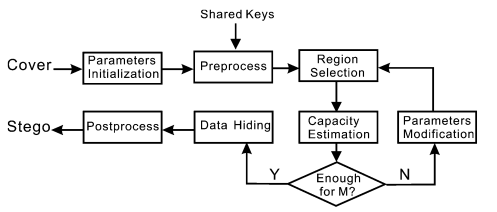
\includegraphics[width=0.6\textwidth]{images/proposed_scheme.png}
\caption{Proposed Scheme (as given in the paper)}
\end{figure}
They use the absolute difference between two adjacent pixels as the criterion for region selection, and use LSBMR as the data hiding algorithm.
\par The {\bf step 1} of the algorithm mainly first divides the whole image into nonoverlapping  blocks of $B_{z}\times B_{z}$ pixels and then rotates each block by $\{0,90,180,270\}$ as determined by a secret key.The resultant image is reshaped into an row vector which is then divided into non overlapping embedding units (two consecutive pixels).
\par {\bf Step 2} calculates the threshold $T$ for region selection using given formula.
\par {\bf Step 3}  Implements data hiding according to four discussed cases.If the modifications are out of constraints then they are readjusted.
\par {\bf Step 4} is similar to step 1 except that the blocks are rotated by same degrees but in opposite direction.
The parameters for $(T,B_{z})$ are hidden in a preset area.

\par {\bf Analysis} - One of the important properties of our steganographic method is that it can first choose the sharper edge regions for data hiding according to the size of the secret message by adjusting a threshold $T$.
The experimental resuls are  summarized in table3 for different embedding rates  in the paper itself show that it has the minimum accuracy of being detected in most of the cases amongst the seven steganographic algorithms.

\newpage
\section{Paper Comprehension by Member 3 - Vedansh Gupta}
In this
paper, we expand the LSB matching revisited image steganography propose an edge adaptive scheme which can select the
embedding regions according to the size of secret message and the difference between two consecutive pixels in the cover image.For lower embedding rates, only sharper edge regions are used while keeping the other smoother regions as they are.
LSB replacement is a well-known steganographic method. In
this embedding scheme, only the LSB plane of the cover image
is overwritten with the secret bit stream according to a pseudorandom
number generator (PRNG). \par LSB matching (LSBM) employs a minor modification to LSB
replacement. If the secret bit does not match the LSB of the
cover image, then $\pm 1$ is randomly added to the corresponding
pixel value. The experimental results demonstrated that
the method was more effective on uncompressed grayscale im
ages. \par LSB matching revisited (LSBMR) uses a pair of pixels as an embedding unit, in which the LSB
of the first pixel carries one bit of secret message, and the relationship
(odd–even combination) of the two pixel values carries
another bit of secret message. In such a way, the modification
rate of pixels can decrease from 0.5 to 0.375 bits/pixel
(bpp) in the case of a maximum embedding rate, meaning fewer
changes to the cover image at the same payload compared to
LSB replacement and LSBM. The typical LSB-based approaches, including LSB replacement,
LSBM, and LSBMR, deal with each given pixel/pixelpair
without considering the difference between the pixel and
its neighbors. \par The pixel-value differencing (PVD)-based scheme
 is another kind of edge adaptive scheme, in
which the number of embedded bits is determined by the difference
between a pixel and its neighbor. The larger the difference,
the larger the number of secret bits that can be embedded.
Usually, PVD-based approaches can provide a larger
embedding capacity. \par Generally, the regions
located at the sharper edges present more complicated statistical
features and are highly dependent on the image contents.
Moreover, it is more difficult to observe changes at the sharper
edges than those in smooth regions. \par For LSB replacement, the secret bit
simply overwrites the LSB of the pixel, i.e., the first bit plane,
while the higher bit planes
are preserved. For the LSBM
scheme, if the secret bit is not equal to the LSB of the given
pixel, then
1 is added randomly to the pixel while keeping the
altered pixel in the range of $[0, 255]$. 

\par
Our human vision is sensitive to slight changes in the smooth
regions, while it can tolerate more severe changes in the edge
regions.The
basic idea of PVD-based approaches is to first divide the cover
image into many nonoverlapping units with two consecutive
pixels and then deal with the embedding unit along a pseudorandom
order which is also determined by a PRNG.
The larger the difference between the two pixels, the larger the number of
secret bits that can be embedded into the unit.

\par We find that uncompressed natural images usually
contain some flat regions (it may be as small as 5X5 and it
is hard to notice), If we embed data into these regions, the LSB of stego images would become more and more random.
Our proposed
scheme will first embed the secret bits into edge regions as far
as possible while keeping other smooth regions as they are.
We have not much focused on the security and safety of our data and image.
In this paper, we apply such a region adaptive scheme to the
spatial LSB domain. We use the absolute difference between
two adjacent pixels as the criterion for region selection, and use
LSBMR as the data hiding algorithm. We have taken two parameters for data hiding approach. The first one is the block size for block dividing in data preprocessing;
another is the threshold for embedding region selection.
\par 
The larger the
number of secret bits to be embedded, the smaller the threshold T
becomes, which means that more embedding units with
lower gradients in the cover image can be released.

When is 0, all the embedding units within the cover become
available. In such a case, our method can achieve the maximum
embedding capacity of 100 \%.

\section{Conclusions and Results}
We conclude the report by saying that what we aimed at while implemenenting the paper has been achieved. We ought to target image steganography and for that we tried using edge adaptive techniques. Although, the author of the code did not implemented the paper in its full essence but the code is working as expected by the author. Few points that must be noted about what implementations have been achieved and what has been not before we conclude with the results. Note: The code has been authored by Himanshu Sharma (Member - 1). \newpage

\underline{\large What has been achieved in the Python code base}
\begin{enumerate}
\item Graphical User Interface has been developed so that anyone can use this software piece.
\item Division of image into blocks of dimension $B \times B$ and then their random rotations has been implemented so as to increase the security as given in the paper.
\item Bit Planes were implemented as they were given in the paper. A special Python script is dedicated for this only.
\item LSB Matching algorithm as given in the paper has been implemented successfully.
\item Image steganography has been done successfully.
\end{enumerate}
\par
\underline{\large What the author was unable to implement in the code}
\begin{enumerate}
\item Because the ``argmin" and ``argmax" operations seemed difficult and therefore steps 2 and 3 of the algorithm (refer the paper) suggested in the paper were not implemented precisely. Instead, a linear form of steganography was done as a substitute to these steps.
\end{enumerate}
If we have to summarize, we summarize the results by operating on the popular test image used in the field of image processing, i.e., the photograph of popular model lenna.
\begin{figure}[H]
\centering
\begin{minipage}{0.46\linewidth}
\centering
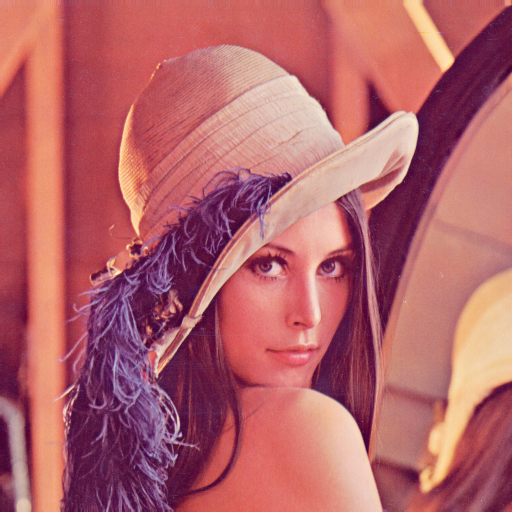
\includegraphics[width=0.7\textwidth]{images/lenna.png}
\caption{Cover Image}
\end{minipage}
\hfill
\begin{minipage}{0.46\linewidth}
\centering
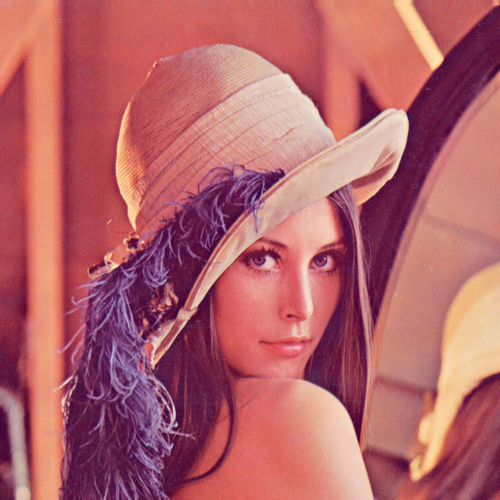
\includegraphics[width=0.7\textwidth]{images/stego-lenna.png}
\caption{Stego Image}
\end{minipage}
\end{figure}
Clearly, there is no difference in the cover and the stego image. Just to convey the information, I am also showing the MSB and LSB planes of the cover and the stego-image.
\begin{figure}[H]
\centering
\begin{minipage}{0.46\linewidth}
\centering
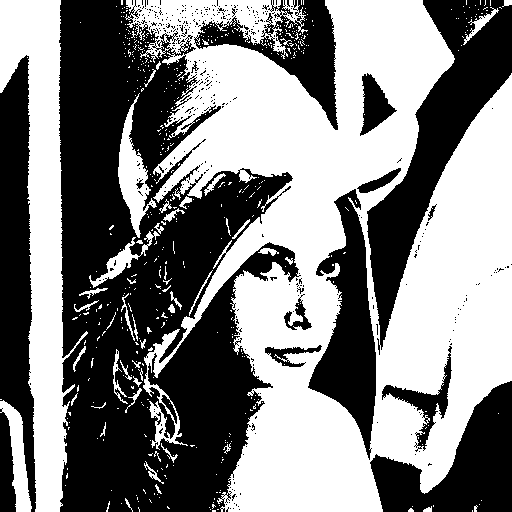
\includegraphics[width=0.7\textwidth]{images/covermsb.png}
\caption{MSB plane of the Cover}
\end{minipage}
\hfill
\begin{minipage}{0.46\linewidth}
\centering
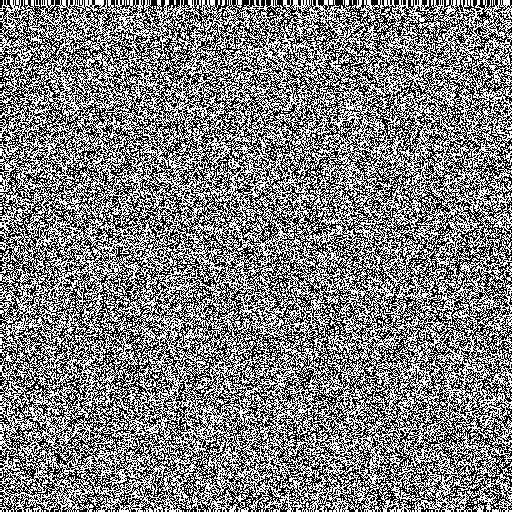
\includegraphics[width=0.7\textwidth]{images/coverlsb.png}
\caption{LSB plane of the Cover}
\end{minipage}
\end{figure}

\begin{figure}[H]
\centering
\begin{minipage}{0.46\linewidth}
\centering
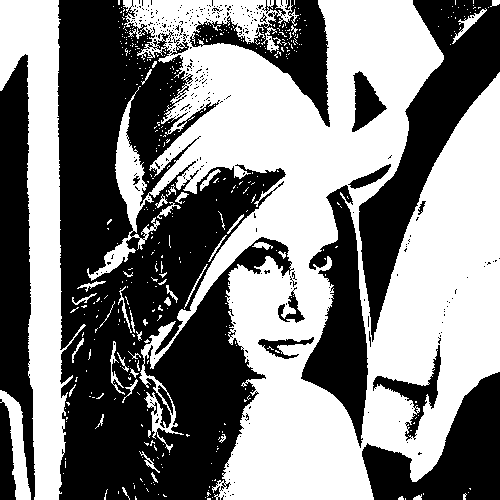
\includegraphics[width=0.7\textwidth]{images/stegomsb.png}
\caption{MSB plane of the Stego}
\end{minipage}
\hfill
\begin{minipage}{0.46\linewidth}
\centering
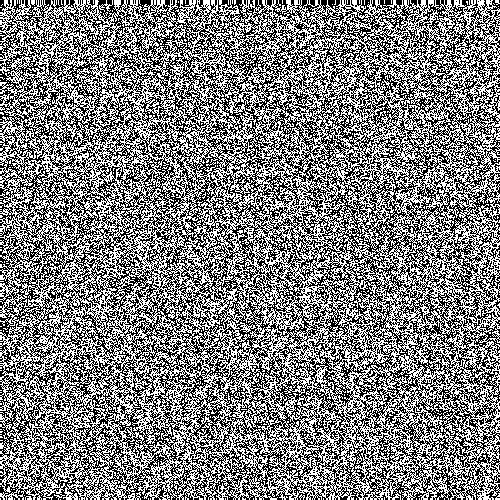
\includegraphics[width=0.7\textwidth]{images/stegolsb.png}
\caption{LSB plane of the Stego}
\end{minipage}
\end{figure}
We conclude by saying that image steganography has been implemented successfully and we got the results as expected.
\\
\par \begin{center} \textbf{IMPORTANT NOTE} \end{center}
\par Full code base is available at Member 1's Github repository - {\bf https://github.com/hmnhGeek/DSP-Project-Report-LaTeX}. We request the reader to please visit and see the code base for atleast once.

\begin{center}
\decosix\decosix\decosix
\end{center}
\end{document}